\paragraph{異方性媒質}
異方性のある媒質中で任意の方向へ進む光について考える.

異方性媒質の誘電率テンソルは一般に,
\begin{align}
  \begin{pmatrix}
    \varepsilon_{11} & \varepsilon_{12} & \varepsilon_{13}\\
    \varepsilon_{21} & \varepsilon_{22} & \varepsilon_{21}\\
    \varepsilon_{31} & \varepsilon_{32} & \varepsilon_{33}
  \end{pmatrix}
\end{align}
と書くことができる.ここで,物質に対し適当な座標系を選ぶと,誘電率テンソルの対角成分以外を0にすることが可能な場合がある.
この場合の座標軸をテンソルの主軸と言い,対角成分を主値と言う.ここで,主軸と主値は物体固有のものである.

主値のうち,2つが一致している時を1軸性の異方性と言い,異なる主値を持つ成分の軸を光学軸と言う.主値がどれも一致していない時は2軸性の異方性と呼ぶ.
以下では媒質が透明で,透磁率が等方的で$\mu$の場合を考える.

Maxwell方程式から,平面波について
\begin{align}
  \rot\boldsymbol{E}&=\boldsymbol{k}\times\boldsymbol{E}=\omega\mu\boldsymbol{H}\label{aniso_kE}\\
  \rot\boldsymbol{H}&=\boldsymbol{k}\times\boldsymbol{H}=-\omega\boldsymbol{D}=-\omega\varepsilon\boldsymbol{E}\label{aniso_kH}
\end{align}
となる.
Poyntingベクトル$\boldsymbol{S}$は\eqref{aniso_kE}\eqref{aniso_kH}から,
\begin{align}
  \boldsymbol{S}=\boldsymbol{E}\times\boldsymbol{H}=\dfrac{1}{\mu\omega}\left[E^2\boldsymbol{k}-(\boldsymbol{k}\cdot\boldsymbol{E})\boldsymbol{E}\right]
\end{align}
で表される.このように,異方性媒質中では波の伝播方向とエネルギーの流れる方向が異なっている.
以上から,$\boldsymbol{k}$, $\boldsymbol{E}$, $\boldsymbol{D}$, $\boldsymbol{H}$, $\boldsymbol{S}$の関係は図のようになる.
$\boldsymbol{k}$, $\boldsymbol{E}$, $\boldsymbol{D}$, $\boldsymbol{S}$は同一平面内に存在する.
さらに,$\boldsymbol{H}$はこの平面に直交する.

\begin{figure}[ht]
  \centering
  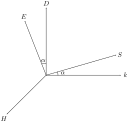
\includegraphics[scale=0.5]{vectors.pdf}
  \caption{主要なベクトルの関係図}
  \label{vectors}
\end{figure}

ここで,
\begin{align}
  \boldsymbol{n}=\dfrac{c}{\omega}\boldsymbol{k}\label{aniso_nvec}
\end{align}
で屈折率ベクトル$\boldsymbol{n}$を定義する.$c$は真空中の光速である.ただし,屈折率ベクトルの絶対値はその向きによって変わる.
また,\eqref{aniso_kE}\eqref{aniso_kH}から,
\begin{align}
  \sum_j(n^2\delta_{ij}-n_i{}n_j-\mu{}c^2\varepsilon_{ij})E_j=0\label{aniso_fresE}
\end{align}
となる.ただし,$\delta_{ij}$はクロネッカーのデルタである.これが$\boldsymbol{E}=0$以外の解を持つには,
\begin{align}
  \text{det}(n^2\delta_{ij}-n_i{}n_j-\mu{}c^2\varepsilon_{ij})=0
\end{align}
であればよい.これを計算するときはテンソルの主軸となる座標系へ移行すると楽である.これを展開すると,6次の項はなくなり,
\begin{align}
  n^2(\varepsilon_{\xi}{n_\xi}^2+\varepsilon_{\eta}{n_\eta}^2+\varepsilon_{\zeta}{n_\zeta}^2)
  -\mu{c}^2\left[{n_\xi}^2\varepsilon_\xi(\varepsilon_\eta+\varepsilon_\zeta)
  +{n_\eta}^2\varepsilon_\eta(\varepsilon_\zeta+\varepsilon_\xi)
  +{n_\zeta}^2\varepsilon_\zeta(\varepsilon_\eta+\varepsilon_\xi)\right] \notag \\
  +\mu^2{c}^4\varepsilon_\xi\varepsilon_\eta\varepsilon_\zeta = 0 . \label{aniso_fresEq}
\end{align}
ただし,テンソルの主値$\varepsilon_{ii}$を$\varepsilon_{i}$とした.これをFresnel方程式と呼ぶ.
Fresnel方程式\eqref{aniso_fresEq}は$n_\xi$, $n_\eta$, $n_\zeta$座標で4次曲面をなす.これを屈折率ベクトル面と呼ぶ.
屈折率ベクトル面は\eqref{aniso_fresEq}から分かるように$\omega$にも依存している.
そして,$\boldsymbol{n}$の方向が決まっている時は\eqref{aniso_fresEq}は$n$に関する2次方程式となるので,一般に2つの解を持つ.
つまり,$\boldsymbol{n}$の方向が決まっている時はその絶対値は2つ存在するということが分かる.

さらに,等方性媒質の中では群速度$\boldsymbol{v}_s$と波数$\boldsymbol{k}$の向きは一致しているが,異方性媒質では一致していない.
異方性媒質中では群速度が光線の方向と一致している.そこで,向きが群速度の向きと一致しており,大きさが
\begin{align}
  \boldsymbol{s}\cdot\boldsymbol{n}=1 \label{aniso_def_s}
\end{align}
となる光線ベクトル$\boldsymbol{s}$を定義する.

\eqref{aniso_kE}\eqref{aniso_kH}\eqref{aniso_nvec}から,
\begin{align}
  \boldsymbol{n}\times\boldsymbol{E} &= \mu{c}\boldsymbol{H}\label{aniso_nE}\\
  \boldsymbol{n}\times\boldsymbol{H} &= -c\boldsymbol{D}\label{aniso_nH}
\end{align}
となる.\eqref{aniso_nE}\eqref{aniso_nH}と定義$\boldsymbol{s}\cdot\boldsymbol{n}=1$から,
\begin{align}
  \boldsymbol{s}\times\boldsymbol{D} &= \boldsymbol{s}\times\left[-\dfrac{1}{c}\boldsymbol{n}\times\boldsymbol{H}\right]\notag\\
  &= -\dfrac{1}{c}\left[(\boldsymbol{s}\cdot\boldsymbol{H})\boldsymbol{n}-(\boldsymbol{s}\cdot\boldsymbol{n})\boldsymbol{H}\right]\notag\\
  &= \dfrac{\boldsymbol{H}}{c} . \label{aniso_sxD}
\end{align}
同様に,
\begin{align}
  \boldsymbol{s}\times\boldsymbol{H}=-\dfrac{1}{\mu{}c}\boldsymbol{E}\label{aniso_sxH}
\end{align}
となる.
\eqref{aniso_sxD}\eqref{aniso_sxH}から,Fresnel方程式を導いたのと同様の議論から,
\begin{align*}
  \text{det}\left(\delta_{ij}s^2\varepsilon_{ij}-\dfrac{\delta_{ij}}{\mu{}c^2}-s_is_j\varepsilon_{ij}\right)=0
\end{align*}
となり,これを展開すると,
\begin{align}
  s^2(\varepsilon_\eta\varepsilon_\zeta{s_\xi}^2+\varepsilon_\zeta\varepsilon_\xi{s_\eta}^2+\varepsilon_\xi\varepsilon_\eta{s_\zeta}^2)
  -\dfrac{1}{\mu{}c^2}\left[{s_\xi}^2(\varepsilon_\eta+\varepsilon_\zeta)+{s_\eta}^2(\varepsilon_\zeta+\varepsilon_\xi)+{s_\zeta}^2(\varepsilon_\xi+\varepsilon_\eta)\right]
  +\dfrac{1}{\mu^2c^4}=0
\end{align}
となる.これを光線速度面方程式と呼ぶ.ただし,主値の添字は略した.これは$(s_\xi,s_\eta,s_\zeta)$座標において4次曲面をなす.これを光線速度面と呼ぶ.

さて,波動光学の近似として幾何光学が有効なのは,問題にしているスケールが波長$\lambda$より十分大きい時だけ.
この条件の下,位置や時間による誘電率の変化は緩やかで,位相は屈折率を光の進路にそって積分した光路長によって表すことができるとする近似をアイコナール近似と呼ぶ.
アイコナール近似では,電場や磁場が
\[\psi(\boldsymbol{r})=a(\boldsymbol{r})\exp[i(k\phi(\boldsymbol{r})-\omega{}t)]\]
と表される時,この$\phi(\boldsymbol{r})$をアイコナールと呼ぶ.
定義と\eqref{aniso_nvec}から,
\begin{align}
  \grad\phi(\boldsymbol{r}) = \boldsymbol{n}.\label{aniso_gradphi}
\end{align}

次に等位相面について考える.アイコナールを含んだ位相は$k\phi-\omega{t}$であるので,ある時刻$t_0$において,
\begin{align}
  \phi = \phi_0 = \text{const}.
\end{align}
で決定される曲面が等位相面である.さらに,微小時間$\delta{t}$経過した後,この等位相面は,
\begin{align}
  k\phi_0-\omega{t_0}=k(\phi_0+\delta\phi)-\omega(t_0+\delta{t})\label{aniso_phidev}
\end{align}
で与えられる$\delta\phi$を用いて,
\begin{align}
  \phi=\phi_0+\delta\phi.
\end{align}
また,\eqref{aniso_phidev}から,
\begin{align}
  \delta\phi=\dfrac{\omega}{k}\delta{t}.
\end{align}
一般に,曲面$\phi(\xi,\eta,\zeta)=\phi_0$上の1点P$_0(\xi_0,\eta_0,\zeta_0)$の近くにP$(\xi_0+\delta\xi,\eta_0+\delta\eta,\zeta_0+\delta\zeta)$を取る.
P$_0$及びPは共に等位相面上にあるので,
\[\phi(\xi_0,\eta_0,\zeta_0)=\phi(\xi_0+\delta\xi,\eta_0+\delta\eta,\zeta_0+\delta\zeta)=\phi_0.\]
最左辺を展開して1次まで取ると,中辺と合わせて,
\[\dfrac{\partial\phi}{\partial\xi}\delta\xi+\dfrac{\partial\phi}{\partial\eta}\delta\eta+\dfrac{\partial\phi}{\partial\zeta}\delta\zeta=0.\]
よって,等位相面内の任意の微小ベクトルを$\delta{\boldsymbol{r}}=(\delta\xi,\delta\eta,\delta\zeta)$を用いると,\eqref{aniso_gradphi}と合わせて,
\begin{align}
  \text{grad}\,\phi(\boldsymbol{r})\cdot\delta\boldsymbol{r}=\boldsymbol{n}\cdot\delta\boldsymbol{r}=0.\label{aniso_ndr}
\end{align}
よって,$(\xi,\eta,\zeta)$座標において屈折率ベクトル$\boldsymbol{n}$は等位相面に対し直交する事が分かる.

% <!--
%
% Fermatの原理から,空間内のある点Aから別の点Bへ進む光の経路は,その経路に沿っての線積分
% \begin{align}
%   \phi=\int_{\text A}^{\text B}\boldsymbol{n}\cdot{}d\boldsymbol{l}=\int_{\text A}^{\text B}ndl
% \end{align}
% が極小になるという条件で決定される.ところで,では群速度$\boldsymbol{v}_s$と光線の向き$l$は平行なので,
% \begin{align}
%   \phi=\int\boldsymbol{n}\cdot{}d\boldsymbol{l}=\int\boldsymbol{n}\cdot\left(\dfrac{\boldsymbol{s}}{s}dl\right)=\int\dfrac{dl}{s}
% \end{align}
% となる.均質な媒質中では$s$は光線に沿って一定であるので,考えている光の経路の長さを$L$とすると,$\phi=\dfrac{L}{s}$となる.これから明らかなように,
% 光束の中心から出る各動径方向で$s$に等しい線分の端点が作る曲面は等位相面となる.これを光線速度面と呼ぶ.
%
% -->

\eqref{aniso_fresEq}のFresnel方程式は$n_i$を使って記述されているが,屈折率ベクトル面を$f(k_\xi,k_\eta,k_\zeta,\omega)=0$で記述することにすると,偏微分の一般的な公式\footnote{\(f=f(k, \omega)\)を変形して\(\omega=\Omega(f, k)\)とする.\(\omega = \Omega(f(k, \omega), k)\)となる.両辺を\(k\)で偏微分すれば\(0 = (\partial\Omega/\partial f)(\partial f/\partial k) + (\partial\Omega/\partial k)\)}から
\[
(v_s)_i = \left( \dfrac{\partial\omega}{\partial{}k_i} \right)_f
= -\dfrac{\left(\cfrac{\partial{f}}{\partial{}k_i}\right)_\omega}{\left(\cfrac{\partial{}f}{\partial\omega}\right)_{k_i}}
= -\dfrac{c}{\omega}\dfrac{\left(\cfrac{\partial{f}}{\partial{}n_i}\right)_\omega}{\left(\cfrac{\partial{}f}{\partial\omega}\right)_{k_i}}
\]
となる.最後の式に移るときは,$\omega$一定という条件で偏微分していることを利用した.
ところで,$\dfrac{\partial{f}}{\partial\boldsymbol{n}}$は曲面$f=0$の法線方向を向いている.
よって,光線ベクトル$\boldsymbol{s}$は屈折率ベクトル面の対応する点における法線の向きを向いていることが分かる.
屈折率ベクトル面は$(n_\xi,n_\eta,n_\zeta)$座標において定義されていることに注意.これは
\begin{align}
  \boldsymbol{s}\cdot\delta\boldsymbol{n}=0\label{aniso_sdn}
\end{align}
と表される.さらに,$\boldsymbol{s}$の定義$\boldsymbol{s}\cdot\boldsymbol{n}=1$を$\omega=\text{const}$の下で両辺微分して,
$\boldsymbol{s}\cdot\delta\boldsymbol{n}+\boldsymbol{n}\cdot\delta\boldsymbol{s}=0$となるので,\eqref{aniso_sdn}から,
\begin{align}
  \boldsymbol{n}\cdot\delta\boldsymbol{s}=0.\label{aniso_nds}
\end{align}
\eqref{aniso_ndr}\eqref{aniso_nds}から,$\delta\boldsymbol{r}$が等位相面内の任意の微小ベクトルであることを考慮すると,$(\xi,\eta,\zeta)$座標において原点から伸ばした光線ベクトル$\boldsymbol{s}$が作る面は等位相面である.
また,\eqref{aniso_nds}から,屈折率ベクトル$\boldsymbol{n}$は光線速度面の対応する点における法線の向きを向いていることが分かる.
光線速度面は$(s_\xi,s_\eta,s_\zeta)$座標において定義されていることに注意.
屈折率ベクトル$\boldsymbol{n}$と同様に,ある1点を出た光であっても,$\boldsymbol{s}$はその向きによって絶対値が変わる.

ここで,Poyntingベクトル$\boldsymbol{S}$と光線ベクトル$\boldsymbol{s}$の関係を求める.\eqref{aniso_kE}と\eqref{aniso_kH}を微分して,
\begin{align*}
  \delta\boldsymbol{D} &= -\dfrac{1}{\omega}[\delta\boldsymbol{k}\times\boldsymbol{H}+\boldsymbol{k}\times\delta\boldsymbol{H}] , \\
  \delta\boldsymbol{H} &= \dfrac{1}{\omega\mu}[\delta\boldsymbol{k}\times\boldsymbol{E}+\boldsymbol{k}\times\delta\boldsymbol{E}] .
\end{align*}
それぞれの両辺で$\boldsymbol{E}$, $\boldsymbol{H}$とのスカラー積を取ると,
\begin{align*}
  \boldsymbol{E}\cdot\delta\boldsymbol{D} = -\dfrac{1}{\omega}[\boldsymbol{E}\cdot(\delta\boldsymbol{k}\times\boldsymbol{H})+\boldsymbol{E}\cdot(\boldsymbol{k}\times\delta\boldsymbol{H})] , \\
  \mu\boldsymbol{H}\cdot\delta\boldsymbol{H} = \dfrac{1}{\omega}[\boldsymbol{H}\cdot(\delta\boldsymbol{k}\times\boldsymbol{E})+\boldsymbol{H}\cdot(\boldsymbol{k}\times\delta\boldsymbol{E})] .
\end{align*}
ここで,ベクトル解析の公式
\[a\cdot(b\times{}c)=(a\times{}b)\cdot{}c\]
及び$\varepsilon_{ij}$の対称性から導かれる式
\[\boldsymbol{D}\cdot\delta\boldsymbol{E}=\sum_i\sum_j\varepsilon_{ij}E_j\delta{}E_i=\sum_i\sum_jE_j\varepsilon_{ji}\delta{}E_i=\boldsymbol{E}\cdot\delta\boldsymbol{D}\]
と\eqref{aniso_kE}と\eqref{aniso_kH}を使うと,
\begin{align*}
  \boldsymbol{E}\cdot\delta\boldsymbol{D} = \dfrac{1}{\omega}(\boldsymbol{E}\times\boldsymbol{H})\cdot\delta\boldsymbol{k}+\mu\boldsymbol{H}\cdot\delta\boldsymbol{H}\\
  \mu\boldsymbol{H}\cdot\delta\boldsymbol{H} = \dfrac{1}{\omega}(\boldsymbol{E}\times\boldsymbol{H})\cdot\delta\boldsymbol{k}+ \boldsymbol{E}\cdot\delta\boldsymbol{D}
\end{align*}
となる.この2式から,$\boldsymbol{k}\parallel\boldsymbol{n}$を考慮すると,
\begin{align}
  (\boldsymbol{E}\times\boldsymbol{H})\cdot\delta\boldsymbol{n}=\boldsymbol{S}\cdot\delta\boldsymbol{n}=0\label{aniso_Sdn}
\end{align}
となる.\eqref{aniso_sdn}\eqref{aniso_Sdn}から,群速度もしくは光線ベクトルとPoyntingベクトルは同じ向きを向いていることが分かる.よって,
\begin{align}
  \boldsymbol{s}\cdot\boldsymbol{H} &= 0\label{aniso_sE}\\
  \boldsymbol{s}\cdot\boldsymbol{E} &= 0.\label{aniso_sH}
\end{align}

異方性媒質中を伝播する光の偏りについて考える.
Fresnel方程式\eqref{aniso_fresEq}を導くきっかけとなった方程式\eqref{aniso_fresE}には電場$\boldsymbol{E}$が含まれている.
だが,$\boldsymbol{k}$と$\boldsymbol{E}$は異なる方向を向いているので,光波の偏りを考えるのには適していない.
図を見ると,$\boldsymbol{k}$と電束密度$\boldsymbol{D}$が直交している.
なので,電束密度$\boldsymbol{D}$を基に式を立て直す.\eqref{aniso_nE}\eqref{aniso_nH}から,
\begin{align}
  \boldsymbol{D}=\dfrac{1}{\mu{c}^2}\left[n^2\boldsymbol{E}-(\boldsymbol{n}\cdot\boldsymbol{E})\boldsymbol{n}\right].\label{aniso_newD}
\end{align}
ここで,新しい式を立てる際に,座標軸が屈折率ベクトル$\boldsymbol{n}$もしくは波数$\boldsymbol{k}$の方を向くようにする.
さらに,この座標系の残りの軸を1,2軸とし,$\alpha=1,2$, $\beta=1,2$とする.$\alpha$軸は$\boldsymbol{n}$と直交するので,\eqref{aniso_newD}の$\alpha$成分は
\[D_\alpha=\dfrac{n^2}{\mu{}c^2}E_\alpha\]
となる.さらに,誘電率の2階逆テンソル$\varepsilon_{\alpha\beta}^{-1}$を考え,
\[E_\alpha=\sum_{\beta}\varepsilon_{\alpha\beta}^{-1}D_\beta.\]
これら2式から,
\begin{align}
  D_\alpha-\dfrac{n^2}{\mu{}c^2}\sum_\beta\varepsilon_{\alpha\beta}^{-1}D_\beta=0
\end{align}
もしくは
\begin{align}
  \left(\dfrac{\mu{}c^2}{n^2}\delta_{\alpha\beta}-\varepsilon_{\alpha\beta}^{-1}\right)D_\beta=0
\end{align}
となる.これはテンソルの固有値問題となっていて,あらわに書けば,
\begin{align}
  \begin{pmatrix}
    \varepsilon^{-1}_{11}-\left(\dfrac{\mu{c^2}}{n^2}\right) & \varepsilon^{-1}_{12}\\
    \varepsilon^{-1}_{21} & \varepsilon^{-1}_{22}-\left(\dfrac{\mu{c^2}}{n^2}\right)
  \end{pmatrix}
  \begin{pmatrix}
    D_1\\
    D_2
  \end{pmatrix}
  =0\label{aniso_newDeq}
\end{align}
が得られる.$\boldsymbol{D}$などのベクトルと誘電率テンソル$\varepsilon$は座標系によって異なる成分を返すことに注意.

\eqref{aniso_newDeq}が$D_1=D_2=0$以外の解を持つ条件は,行列式が0となることなので,
\begin{align}
  \dfrac{\mu{}c^2}{n^2}=\dfrac{\varepsilon^{-1}_{11}+\varepsilon^{-1}_{22}\pm\sqrt{(\varepsilon^{-1}_{11}-\varepsilon^{-1}_{22})^2+4\varepsilon^{-1}_{12}\varepsilon^{-1}_{21}}}{2}
\end{align}
となる.また,先程も述べたように,$\boldsymbol{n}$の向きが決まっている時,その絶対値$n$は2つ存在する.
この式から,確かに$n$は2つ存在することが分かる.それを$n^{(1)}$, $n^{(2)}$とする.
\eqref{aniso_newDeq}の行列式が0になるという条件はもとの$(\xi,\eta,\zeta)$座標におけるFresnel方程式に一致する.
この座標系は$\varepsilon$の主軸であった.さて,\eqref{aniso_newDeq}を見ると,$n^{(1)}$と$n^{(2)}$に対応する二つの$\boldsymbol{D^{(1)}}$と$\boldsymbol{D^{(2)}}$が存在し,それらは$\varepsilon^{-1}$の固有ベクトル(主軸)である.
一般に,固有ベクトル同士は直交するので,$\boldsymbol{D^{(1)}}$と$\boldsymbol{D^{(2)}}$は$(1,2)$平面内で直交する.
先ほどの固有値問題は2次元テンソルについて考えていたことに注意.
ところが,双方とも$\boldsymbol{n}$に直交する平面つまり$(1,2)$平面内にのみ存在することは分かっているので,結局,
\begin{align}
  \boldsymbol{D^{(1)}}\cdot\boldsymbol{D^{(2)}}=0
\end{align}
となる.同じ向きの屈折率ベクトルを持つ2つの光波の電束密度は互いに直交することが分かった.

\eqref{aniso_newDeq}を幾何的に表す.誘電率テンソルの主軸である$(\xi,\eta,\zeta)$座標における$\varepsilon^{-1}$に対応するテンソル楕円体
\begin{align}
  \sum_i\sum_k\varepsilon^{-1}_{ik}r_ir_k=\mu{c^2}=\dfrac{1}{\varepsilon_0}\label{aniso_tensEll}
\end{align}
を考える.$r_1,r_2,r_3$はそれぞれ$\xi,\eta,\zeta$を示す.$\varepsilon$の主軸は$\varepsilon^{-1}$の主軸にもなるので,$(\xi,\eta,\zeta)$においては
\begin{align}
  \varepsilon^{-1}
  =
  \begin{pmatrix}
    \dfrac{1}{\varepsilon_\xi} & 0 & 0 \\
    0 & \dfrac{1}{\varepsilon_\eta} & 0 \\
    0 & 0 & \dfrac{1}{\varepsilon_\zeta}
  \end{pmatrix}\label{aniso_inverse}
\end{align}
の形で表される.\eqref{aniso_tensEll}を\eqref{aniso_inverse}に代入して,
\begin{align}
  \dfrac{\xi^2}{\varepsilon_\xi/\varepsilon_0}+\dfrac{\eta^2}{\varepsilon_\eta/\varepsilon_0}+\dfrac{\zeta^2}{\varepsilon_\zeta/\varepsilon_0}=1\label{aniso_nEll}
\end{align}
となる.これを屈折率楕円体と呼ぶ.

\begin{figure}[ht]
  \centering
  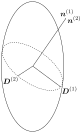
\includegraphics[scale=0.4]{nEllipse.pdf}
  \caption{屈折率楕円体}
  \label{nEllipse}
\end{figure}

屈折率楕円体の$\xi$軸,$\eta$軸,$\zeta$軸との交点の値$\sqrt{\dfrac{\varepsilon_\xi}{\varepsilon_0}}$, $\sqrt{\dfrac{\varepsilon_\eta}{\varepsilon_0}}$, $\sqrt{\dfrac{\varepsilon_\zeta}{\varepsilon_0}}$を主屈折率と呼ぶ.

中心を通り,$\boldsymbol{n}$に垂直な面で屈折率楕円体を切る.この平面の式は,
\begin{align}
  n_\xi\xi+n_\eta\eta+n_\zeta\zeta=0\label{aniso_plane}
\end{align}
で与えられる.切断面の楕円の長軸と短軸を求める.これは,\eqref{aniso_nEll}\eqref{aniso_plane}のもとで
\begin{align}
  r^2=\xi^2+\eta^2+\zeta^2
\end{align}
の極値を求めることに等しい.これにはLagrangeの未定乗数法を使う.
\begin{align}
  F=\xi^2+\eta^2+\zeta^2+2\lambda_1\left(n_\xi\xi+n_\eta\eta+n_\zeta\zeta\right)+\lambda_2\left(\dfrac{\xi^2}{\varepsilon_\xi/\varepsilon_0}+\dfrac{\eta^2}{\varepsilon_\eta/\varepsilon_0}+\dfrac{\zeta^2}{\varepsilon_\zeta/\varepsilon_0}-1\right)
\end{align}
となる$F$に対し,
\begin{align*}
  \dfrac{\partial{F}}{\partial\xi}=2\xi+2\lambda_1n_\xi+2\lambda_2\dfrac{\xi}{\varepsilon_\xi/\varepsilon_0}=0\\
  \dfrac{\partial{F}}{\partial\eta}=2\eta+2\lambda_1n_\eta+2\lambda_2\dfrac{\eta}{\varepsilon_\eta/\varepsilon_0}=0\\
  \dfrac{\partial{F}}{\partial\zeta}=2\zeta+2\lambda_1n_\zeta+2\lambda_2\dfrac{\zeta}{\varepsilon_\zeta/\varepsilon_0}=0
\end{align*}
を解けばよい.これらから,
\begin{align}
  \begin{split}
    \left(1+\dfrac{\lambda_2}{\varepsilon_\xi/\varepsilon_0}\right)\xi+\lambda_1n_\xi=0\\
    \left(1+\dfrac{\lambda_2}{\varepsilon_\eta/\varepsilon_0}\right)\eta+\lambda_1n_\eta=0\\
    \left(1+\dfrac{\lambda_2}{\varepsilon_\zeta/\varepsilon_0}\right)\zeta+\lambda_1n_\zeta=0
  \end{split}
  \label{aniso_lag1}
\end{align}
両辺に$\xi,\eta,\zeta$をかけて足し合わせると,
\begin{align}
  \xi^2+\eta^2+\zeta^2+\lambda_2\left(\dfrac{\xi^2}{\varepsilon_\xi/\varepsilon_0}+\dfrac{\eta^2}{\varepsilon_\eta/\varepsilon_0}+\dfrac{\zeta^2}{\varepsilon_\zeta/\varepsilon_0}\right)+\lambda_1\left(n_\xi\xi+n_\eta\eta+n_\zeta\zeta\right) .
\end{align}
\eqref{aniso_nEll}\eqref{aniso_plane}より,第2項は1,第3項は0となるので,
\begin{align}
  r^2+\lambda_2=0 . \label{aniso_lambda2}
\end{align}
\eqref{aniso_lag1}両辺に$n_\xi,n_\eta,n_\zeta$をかけて足し合わせると,
\begin{align*}
  \left(n_\xi\xi+n_\eta\eta+n_\zeta\zeta\right) + \lambda_2\left(\dfrac{n_\xi\xi}{\varepsilon_\xi/\varepsilon_0}
  + \dfrac{n_\eta\eta}{\varepsilon_\eta/\varepsilon_0} + \dfrac{n_\zeta\zeta}{\varepsilon_\zeta/\varepsilon_0}\right)
  +\lambda_1\left({n_\xi}^2+{n_\eta}^2+{n_\zeta}^2\right) = 0 .
\end{align*}
\eqref{aniso_plane}より,第1項は0となり,第3項は$n^2$となるので,
\begin{align*}
  \lambda_1+\dfrac{\lambda_2}{n^2}\left(\dfrac{n_\xi\xi}{\varepsilon_\xi/\varepsilon_0}+\dfrac{n_\eta\eta}{\varepsilon_\eta/\varepsilon_0}+\dfrac{n_\zeta\zeta}{\varepsilon_\zeta/\varepsilon_0}\right)=0 .
\end{align*}
\eqref{aniso_lambda2}と合わせると,
\begin{align}
  \lambda_1=\dfrac{r^2}{n^2}\left(\dfrac{n_\xi\xi}{\varepsilon_\xi/\varepsilon_0}+\dfrac{n_\eta\eta}{\varepsilon_\eta/\varepsilon_0}+\dfrac{n_\zeta\zeta}{\varepsilon_\zeta/\varepsilon_0}\right) . \label{aniso_lambda1}
\end{align}
\eqref{aniso_lambda2}と\eqref{aniso_lambda1}を\eqref{aniso_lag1}に代入すると,
\begin{align}
  \begin{split}
    \left(1-\dfrac{r^2}{\varepsilon_\xi/\varepsilon_0}\right)\xi+n_\xi\dfrac{r^2}{n^2}\left(\dfrac{n_\xi\xi}{\varepsilon_\xi/\varepsilon_0}
    + \dfrac{n_\eta\eta}{\varepsilon_\eta/\varepsilon_0}+\dfrac{n_\zeta\zeta}{\varepsilon_\zeta/\varepsilon_0}\right)=0 , \\
    \left(1-\dfrac{r^2}{\varepsilon_\eta/\varepsilon_0}\right)\eta+n_\eta\dfrac{r^2}{n^2}\left(\dfrac{n_\xi\xi}{\varepsilon_\xi/\varepsilon_0}
    + \dfrac{n_\eta\eta}{\varepsilon_\eta/\varepsilon_0}+\dfrac{n_\zeta\zeta}{\varepsilon_\zeta/\varepsilon_0}\right)=0 , \\
    \left(1-\dfrac{r^2}{\varepsilon_\zeta/\varepsilon_0}\right)\zeta+n_\zeta\dfrac{r^2}{n^2}\left(\dfrac{n_\xi\xi}{\varepsilon_\xi/\varepsilon_0}
    + \dfrac{n_\eta\eta}{\varepsilon_\eta/\varepsilon_0}+\dfrac{n_\zeta\zeta}{\varepsilon_\zeta/\varepsilon_0}\right)=0 .
  \end{split}\label{aniso_r}
\end{align}
\eqref{aniso_newD}は
\[
\boldsymbol{D}-\dfrac{1}{\mu{c}^2}\left[n^2\boldsymbol{E}-(\boldsymbol{n}\cdot\boldsymbol{E})\boldsymbol{n}\right]
= \boldsymbol{D}-\varepsilon_0n^2\boldsymbol{E}+\varepsilon_0(\boldsymbol{n}\cdot\boldsymbol{E})\boldsymbol{n} = 0
\]
と書くことができる.これを各成分について書くと,
\begin{align}
  D_i-\varepsilon_0n^2E_i+n_i\varepsilon_0\left(n_\xi{}E_\xi+n_\eta{}E_\eta+n_\zeta{}E_\zeta\right)
  &= \left(1-\dfrac{n^2}{\varepsilon_i/\varepsilon_0}\right)D_i+n_i\left(\dfrac{n_\xi{}D_\xi}{\varepsilon_\xi/\varepsilon_0}+\dfrac{n_\eta{}D_\eta}{\varepsilon_\eta/\varepsilon_0}+\dfrac{n_\zeta{}D_\zeta}{\varepsilon_\zeta/\varepsilon_0}\right)\notag\\
  &=0
\end{align}
となる.よって,これを満たす$(\xi,\eta,\zeta)$で$r$は極値を取る.\eqref{aniso_r}と比較すると,
\[r = n, \quad \xi=D_\xi , \quad \eta=D_\eta , \quad \zeta=D_\zeta\]
とすれば完全に対応する.ただし,$D_i$は定数倍の不定性が残っている.
つまり,屈折率楕円体を中心を通る$\boldsymbol{n}$に垂直な面で切った時の楕円断面の長半径及び短半径は2つの屈折率ベクトルの大きさ$n^{(1)}$, $n^{(2)}$に等しく,
各半径のベクトルは電束密度$\boldsymbol{D}^{(1)}$, $\boldsymbol{D}^{(2)}$の向きを向いていることが分かる.

これと同様に,光線ベクトル$\boldsymbol{s}$を使ってテンソル楕円体を定義することもできる.
\eqref{aniso_sxH}と\eqref{aniso_sxD}から,
\begin{align}
  \boldsymbol{E}=\mu{}c^2\left[s^2\boldsymbol{D}-(\boldsymbol{s}\cdot\boldsymbol{D})\boldsymbol{s}\right]
\end{align}
となる.光線ベクトル$\boldsymbol{s}$を軸とする座標系を考え,残りの軸を1,2軸として$\alpha=1,2$を用いると,
\begin{align}
  E_\alpha=\mu{c^2}s^2D_\alpha
\end{align}
と表すことができる.$\boldsymbol{s}$と$\boldsymbol{E}$が直交していることを用いた.また,2次元2階テンソルとなる誘電率$\varepsilon$を用いて,
\begin{align}
  D_\alpha=\sum_\beta\varepsilon_{\alpha\beta}E_\beta
\end{align}
である.以上から,
\begin{align}
  \begin{pmatrix}
    \varepsilon_{11}-\dfrac{1}{\mu{}c^2s^2} & \varepsilon_{12}\\
    \varepsilon_{21} & \varepsilon_{22}-\dfrac{1}{\mu{}c^2s^2}
  \end{pmatrix}
  \begin{pmatrix}
    E_1 \\
    E_2
  \end{pmatrix}
  =0
\end{align}
となる.これが$\boldsymbol{E}=0$以外の解を持つ条件は,この行列式が0となることである.よって,
\begin{align}
  \dfrac{1}{\mu{}c^2s^2}=\dfrac{\varepsilon_{11}+\varepsilon_{22}\pm\sqrt{(\varepsilon_{11}-\varepsilon_{22})^2+4\varepsilon_{12}\varepsilon_{21}}}{2}
\end{align}
となる.これから分かるように,$\boldsymbol{s}$の向きが決まると,その絶対値$s$は2つ存在する.これらを$\boldsymbol{s}^{(1)}$, $\boldsymbol{s}^{(2)}$とする.
また,$\varepsilon_{\alpha\beta}$の固有値は$\dfrac{1}{\mu{c^2}s^2}$であり,固有ベクトルは$\varepsilon_{E}$である.
固有ベクトル同士は直交するので,$\boldsymbol{s}^{(1)}$, $\boldsymbol{s}^{(2)}$に対応する電場$\boldsymbol{E}^{(1)}$, $\boldsymbol{E}^{(2)}$は同じ平面内に存在することを考慮すると,
3次元の空間においても同じ向きの光線ベクトルを持つ2つの光波の電場は互いに直交することが結論される.

これを幾何的に表現するには,$(1,2,s)$座標系から$(\xi,\eta,\zeta)$座標系に戻って,テンソル楕円体
\begin{align}
  \sum_i\sum_k\varepsilon_{ik}r_ir_k=\varepsilon_0
\end{align}
を考えれば良い.展開すると,
\begin{align}
  \dfrac{\varepsilon_\xi}{\varepsilon_0}\xi^2+\dfrac{\varepsilon_\eta}{\varepsilon_0}\eta^2+\dfrac{\varepsilon_\zeta}{\varepsilon_0}\zeta^2=1
\end{align}
となる.これはFresnel楕円体と呼ばれている.

\begin{figure}[ht]
  \centering
  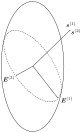
\includegraphics[scale=0.4]{fEllipse.pdf}
  \caption{Fresnel楕円体}
  \label{fEllipse}
\end{figure}

また,先程と同様の議論から,Fresnel楕円体を中心を通り$\boldsymbol{s}$に垂直な面で切った時の楕円断面の長半径及び短半径は2つの光線ベクトルの大きさ$s^{(1)}$, $s^{(2)}$に等しく,
各半径のベクトルは電場$\boldsymbol{E}^{(1)}$, $\boldsymbol{E}^{(2)}$の向きを向いていることが分かる.
また,誘電率が位置によって変化しない均質な物質では,$\boldsymbol{s}$と$\boldsymbol{n}$は変化しないので,2つの楕円体を光と共に動かして考えると,電束密度と電場の方向は常に同じ向きであることが分かる.
つまり,異方性媒質中を伝わる2つの光は直線偏光であることが分かる.

最後に異方性媒質を伝播する光波の重要な性質をいくらかまとめておく.
\begin{enumerate}
  \item $\boldsymbol{E}$, $\boldsymbol{D}$, $\boldsymbol{k}(\boldsymbol{n})$, $\boldsymbol{S}(\boldsymbol{s})$は同一平面内に存在し,$\boldsymbol{H}$はそれに直交する.
  \item 群速度(光線ベクトル)とPoyntingベクトルは同じ向きを向いている.つまり,群速度の向きにエネルギーの伝播が起こっている.
  \item 向きが決まっている群速度(光線ベクトル),波数(屈折率ベクトル)についてはその絶対値が2つ存在する.
  \item (実空間において)屈折率ベクトルは等位相面に直交する.
  \item 光線ベクトルはFresnel方程式から決定される屈折率ベクトル面の法線の向きを向いている.
  % ただし,屈折率ベクトル面は$(n_\xi,n_\eta,n_\zeta)$空間に存在する.
  \item 空間座標において原点から伸ばした光線ベクトルが作る面は等位相面である.
  \item 屈折率ベクトルは光線速度面方程式から決定される光線速度面の法線の向きを向いている.
  % ただし,光線速度面は$(s_\xi,s_\eta,s_\zeta)$空間に存在する.
  \item 同じ向きの屈折率ベクトルを持つ2つの光波の電束密度は直交する.
  \item 同じ向きの光線ベクトルを持つ2つの光波の電場は直交する.
  \item 実空間の屈折率楕円体によって2つの屈折率ベクトルの大きさと電束密度の向きが分かる.
  \item 実空間のFresnel楕円体によって2つの光線ベクトルの大きさと電場の向きが分かる.
  \item 異方性媒質中を伝わる2つの光は直線偏光である
\end{enumerate}
